% Created 2024-07-25 jue 17:43
% Intended LaTeX compiler: pdflatex
\documentclass[presentation]{beamer}
\usepackage[utf8]{inputenc}
\usepackage[T1]{fontenc}
\usepackage{graphicx}
\usepackage{grffile}
\usepackage{longtable}
\usepackage{wrapfig}
\usepackage{rotating}
\usepackage[normalem]{ulem}
\usepackage{amsmath}
\usepackage{textcomp}
\usepackage{amssymb}
\usepackage{capt-of}
\usepackage{hyperref}
\usetheme{default}
\usecolortheme{}
\usefonttheme{}
\useinnertheme{}
\useoutertheme{}
\author{Enrique Perez S}
\date{<2024-07-2>}
\title{Raids}

\hypersetup{
 pdfauthor={Enrique Perez S},
 pdftitle={Raids},
 pdfkeywords={},
 pdfsubject={},
 pdfcreator={Emacs 27.1 (Org mode 9.3)}, 
 pdflang={Spanish}}
\begin{document}

\maketitle
\begin{frame}{Outline}
\tableofcontents
\end{frame}


\section{RAID (7,207,E2)}
\label{sec:org4ddbac1}
\section{Introducción}
\label{sec:org42fa604}
\begin{frame}[label={sec:org542865e}]{Dónde se usan Riads de memoria}
Servidores de almacenamiento
\begin{center}
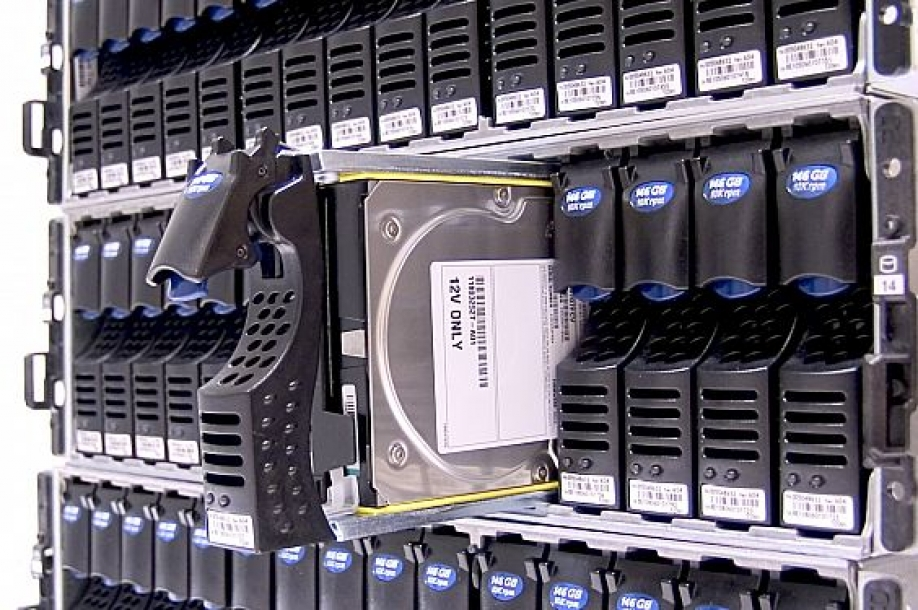
\includegraphics[width=.9\linewidth]{./imagenes/Servidores.jpg}
\end{center}
\end{frame}

\begin{frame}[label={sec:org1efd698}]{Dónde se usan Riads de memoria 2}
NAS (Network-attached storage)
\begin{center}
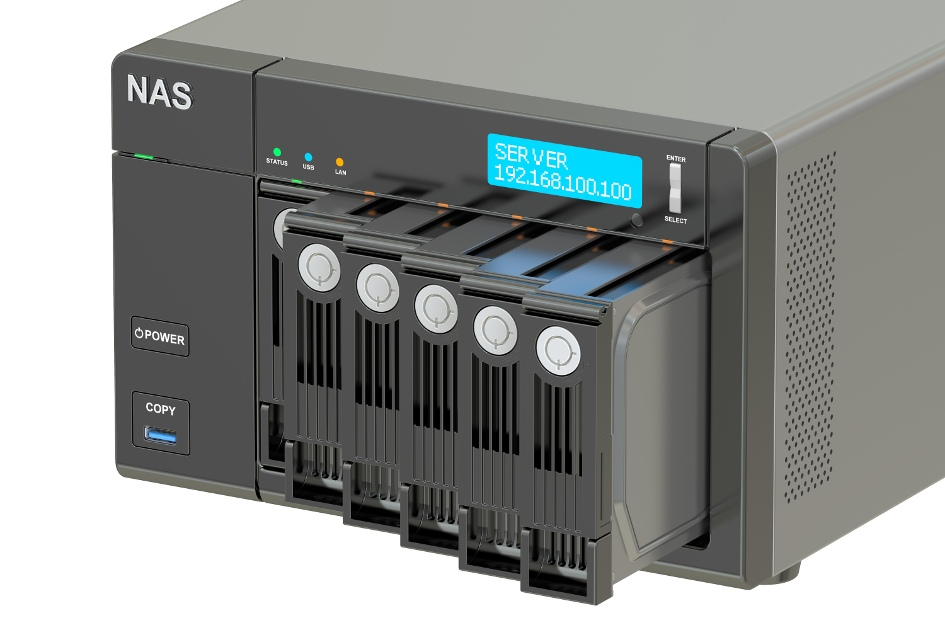
\includegraphics[width=.9\linewidth]{./imagenes/NAS_ejemplo.jpeg}
\end{center}
\end{frame}

\section{Hardware}
\label{sec:org1c5df73}
\begin{frame}[label={sec:org3294242}]{Diferencias entre Hardware}
Los servidores necesitan HDD, SSD y memorias RAM distintos.

HDD - Durabilidad, trabajo continuo, velocidad (10.000 - 15.000 RPM), Memoria Cache 128mb, Interfaces
\begin{center}
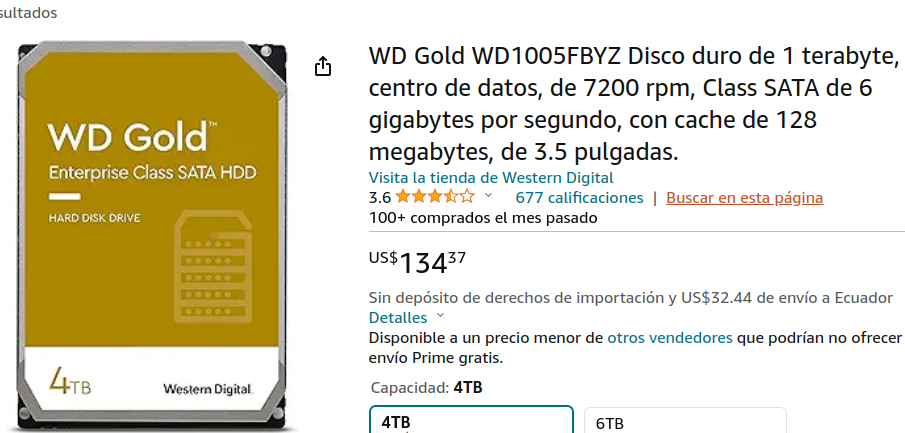
\includegraphics[width=.9\linewidth]{./imagenes/HDD_Servidor.png}
\end{center}
\end{frame}

\begin{frame}[label={sec:orgc5e9bdf}]{Diferencias entre Hardware 2}
SSD de Servidor: Tienen una mayor durabilidad con TBW (Total bytes written) mucho más alto y características adicionales de protección de datos, menor latencia y capacidades que llegan hasta los 15TB.
\begin{center}
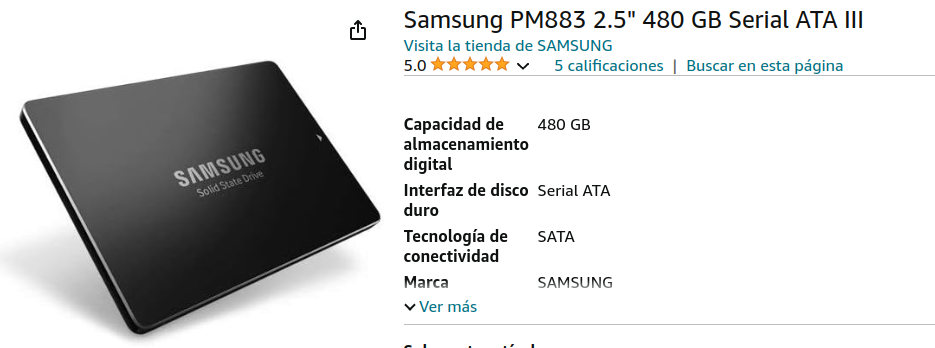
\includegraphics[width=.9\linewidth]{./imagenes/SSDserver.png}
\end{center}
\end{frame}

\begin{frame}[label={sec:orga43213d}]{Diferencias entre Hardware 3}
Memorias Ram: Conocidas como RAM ECC (Error-Correcting Code), tienen mayor fiabilidad y estabilidad que las momorias Ram normales.
\begin{center}
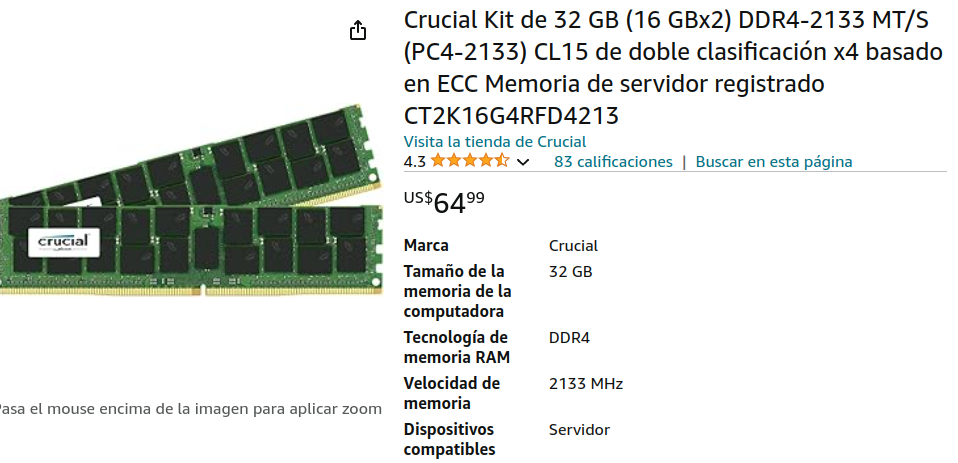
\includegraphics[width=.9\linewidth]{./imagenes/RAMserver.png}
\end{center}
\end{frame}

\section{Comparación.}
\label{sec:orgb1df30f}

\begin{frame}[label={sec:orgfe5a98a}]{Nas}
Un NAS (Network-attached storage) es un equipo especializado en proporcionar el hardware necesario para utilizar la mayor cantidad de dispositivos de almacenamiento (HDD y SSD).

Tiene varias Bahias de discos, principalmente para tamaños de "3.5" pulgadas o "2.5" (laptop).

\begin{center}
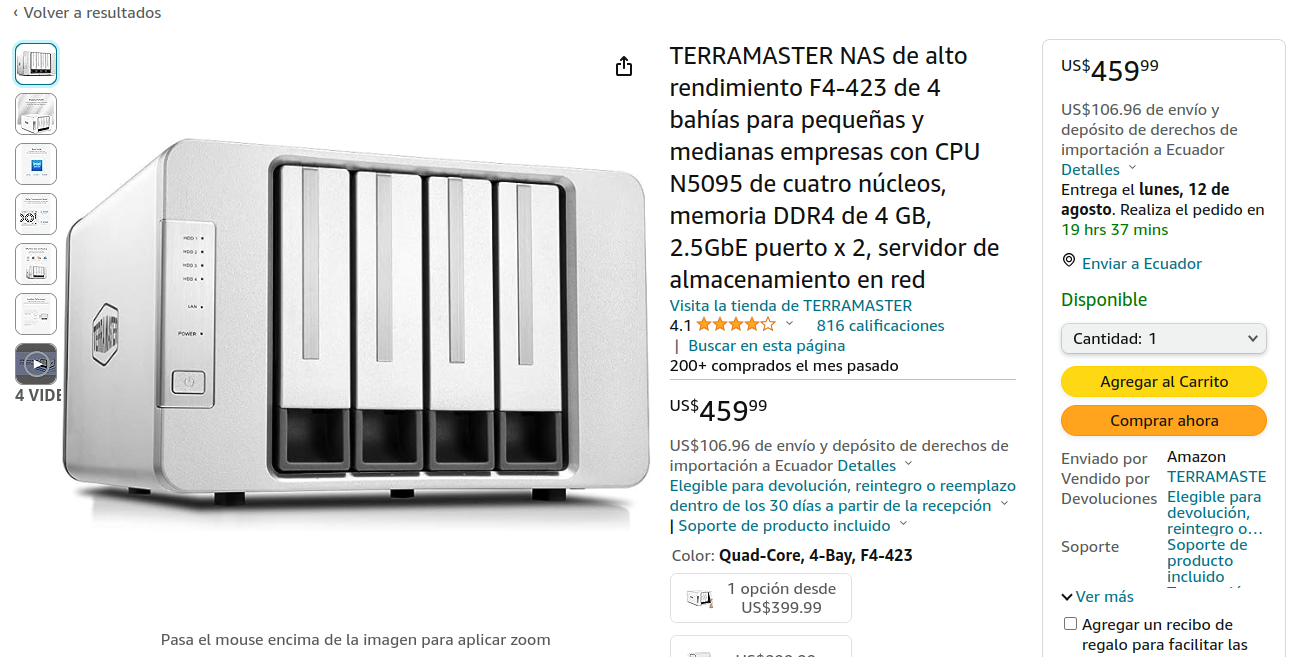
\includegraphics[width=.9\linewidth]{./imagenes/NAS1.png}
\end{center}
\end{frame}

\begin{frame}[label={sec:orgfdf5f77}]{Hardware de NAS 2}
Los NAS tienen los mismos puertos que una computadora normal: Puertos USB, SATA, Ethernet(2.5GB), conector de corriente, etc.

\begin{center}
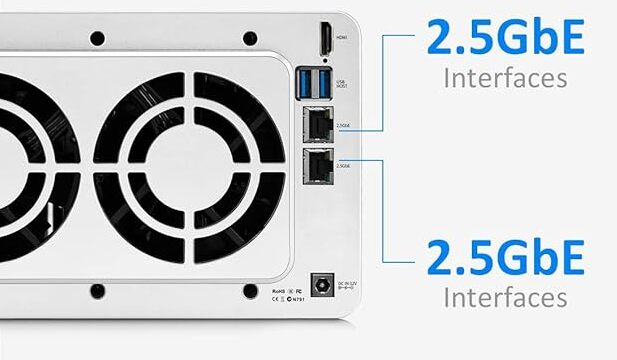
\includegraphics[width=.9\linewidth]{./imagenes/Componentes4.jpg}
\end{center}
\end{frame}

\begin{frame}[label={sec:org5443b39}]{Hardware de NAS 3}
Es una computoradora con chasis especifico para lutilizar facilmente dispositivos de memoria.

En la siguiente comparación vemos el limitado hardware que utiliza.

\begin{center}
\includegraphics[width=.9\linewidth]{./imagenes/Comparación.png}
\end{center}
\end{frame}

\begin{frame}[label={sec:org819488c}]{Hardware de NAS 4}
Los dispositivos NAS más caros tienen mayor cantidad de Bahias de "3.5" y "2.5" y M.2 Nvme junto con conexiones tipo Ethernet 2.5Gb o 10Gb

Si bien todo esto se puede encontrar en otros equipos más económicos, o añadirlos usando Bahías pciex4, los NAS vienen con sistemas operativos especializados para manejar los dispositivos de almacenamiento.

\begin{center}
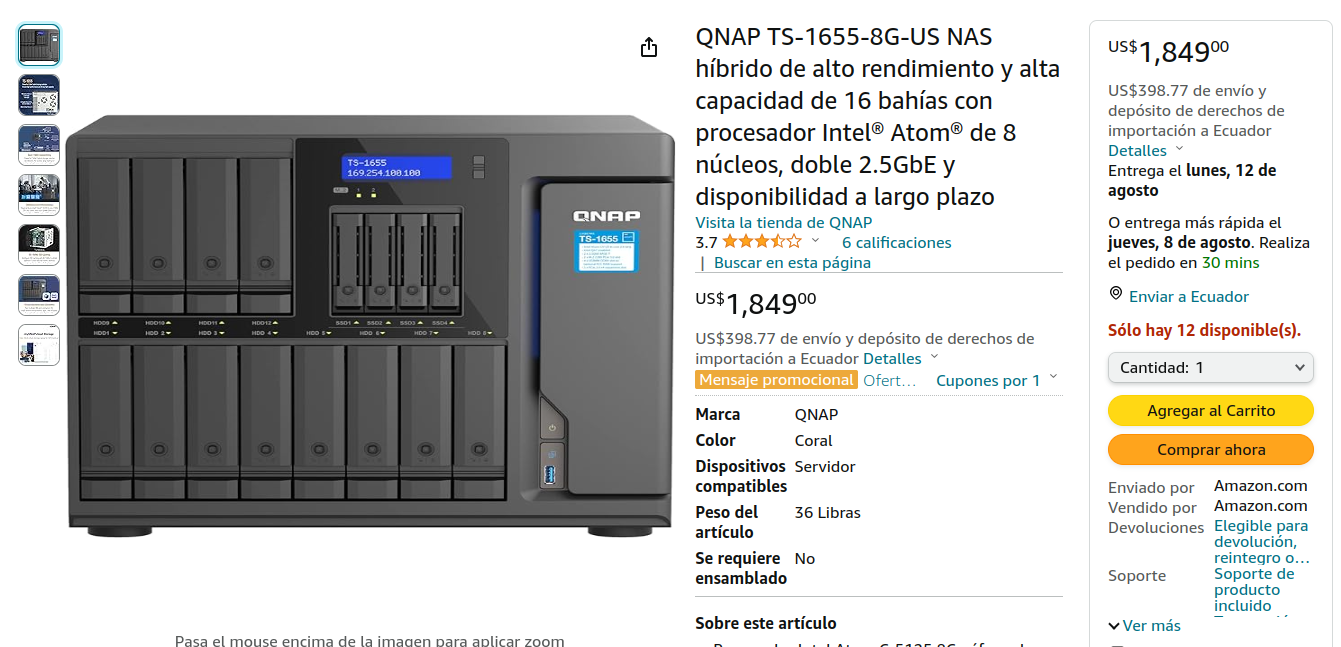
\includegraphics[width=.9\linewidth]{./imagenes/NAS Premium.png}
\end{center}
\end{frame}

\section{Your own NAS}
\label{sec:org256c20a}
\begin{frame}[label={sec:org8578c68}]{PC como NAS}
Como vimos antes, el hardware es el mismo, entonces podemos usar cualquier hardware que tenga la capacidad de conectar discos duros.
\begin{center}
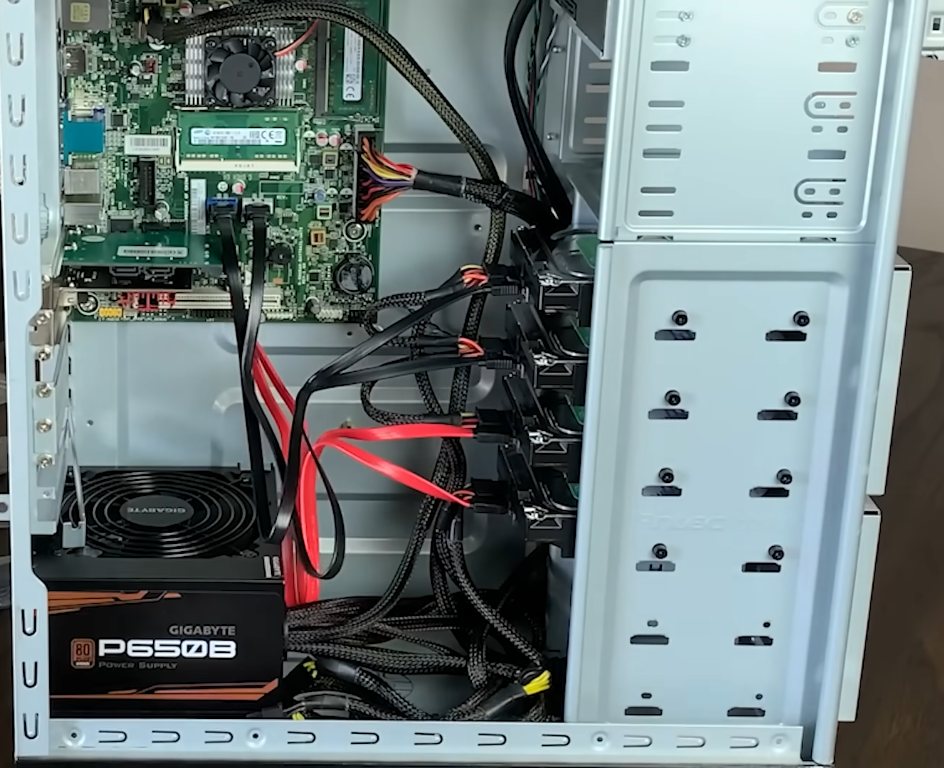
\includegraphics[width=.9\linewidth]{./imagenes/PC.png}
\end{center}
\end{frame}

\begin{frame}[label={sec:orgc112214}]{Sistema operativo para NAS}
Existen multiples sistemas operativos para instalar en tu NAS casero, uno de ellos es TrueNas.

\url{https://www.truenas.com/}
\begin{center}
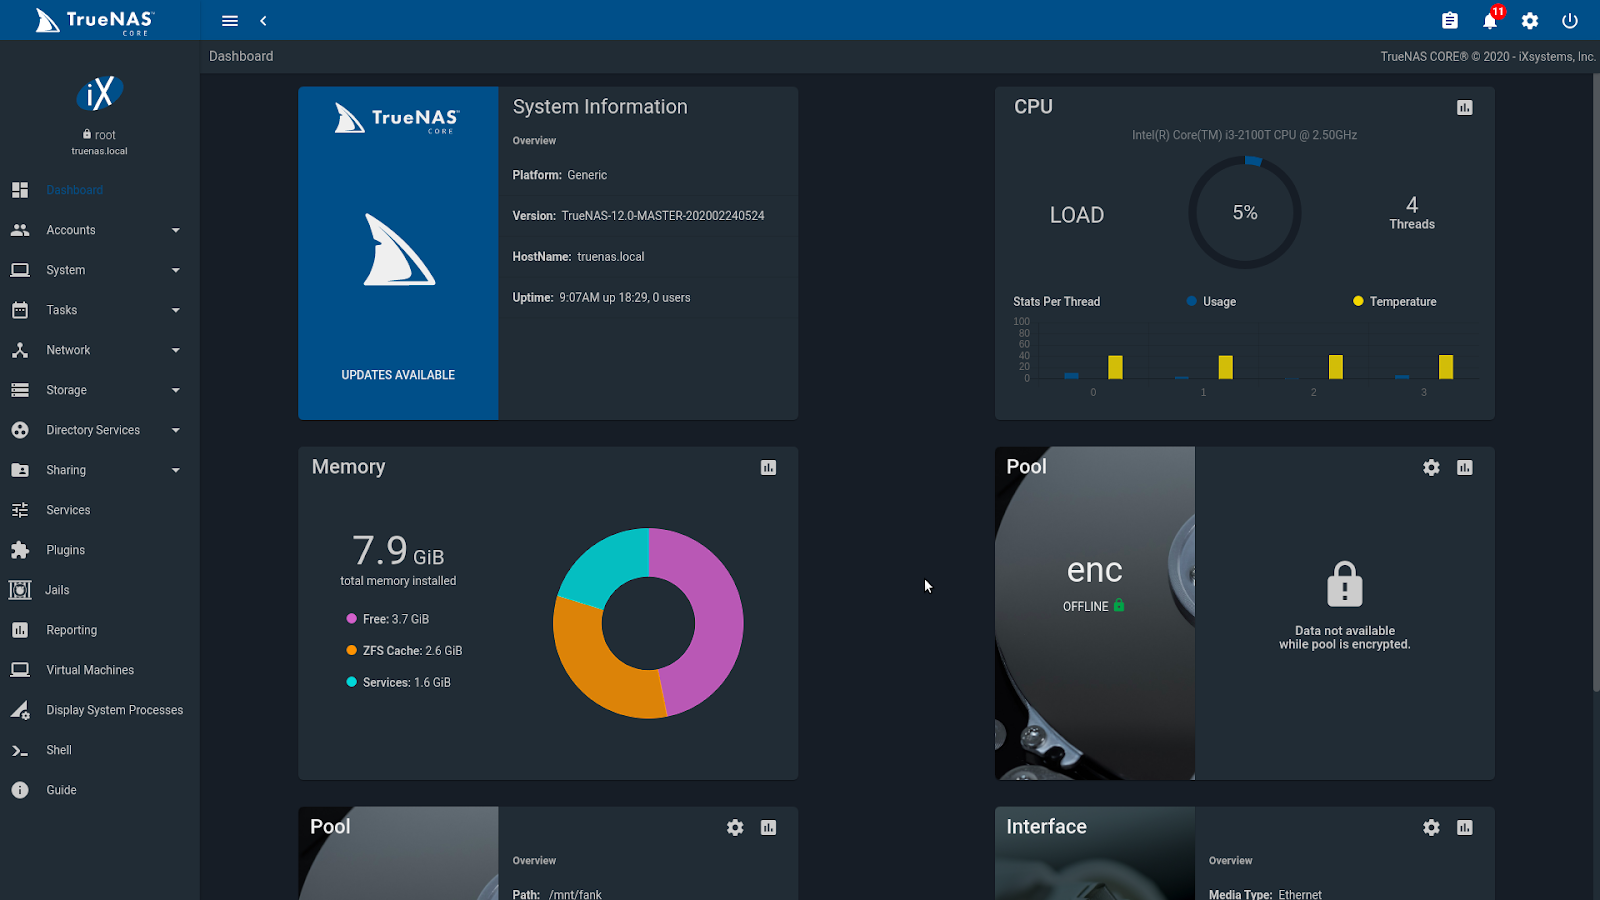
\includegraphics[width=.9\linewidth]{./imagenes/TrueNASSO.png}
\end{center}
\end{frame}

\begin{frame}[label={sec:org2ce9c9c}]{Ventajas de TrueNas y otros SO-NAS}
Las mayores ventajas de los Sistemas operativos para NAS son las funcionalidades para gestionar el almacenamiento.$$\n$$
Dentro del sistema operativo hay herramientas para crear Raids de memoria, servidores de tipo Plex (películas), SMB o Samba (Compartidor de archivos en Windows), etc$$\n$$
Otra de las funcionalidades es agendar copias de seguridad que se realizaran de forma agendada, de tal manera que se creen solo en ciertos periodos de tiempo.$$\n$$
El Sistema operativo también permite crear máquinas virtuales y otras cosas más para crear o levantar servicios, no hay problemas ya que son computadores normales
\end{frame}

\begin{frame}[label={sec:orgb8ef0b7}]{Conclusión}
Los dispositivos NAS se utilizan para poder crear Raids de memoria utilizando los discos duros y discos sólidos conectados.$${\n}$$

Algunos dispositivos NAS tienen un alto costo a pesar de sus limitadas características de Hardware pero se puede crear un NAS propio con el fin de tener un mejor manejo del almacenamiento y mayor seguridad.
\end{frame}
\end{document}
